
\section{Grupo 1 - Cluedo matemático (21/11/2016)}

El primer grupo está formado por:
\begin{itemize}
\item Ana Reyes Camacho 

\item Antonio Jesús Guerrero Lobato 

\item Clara Rocío Lambas Magron 

\item Manuel Pulido Lopez 
\end{itemize}
\begin{figure}[h]
\centering
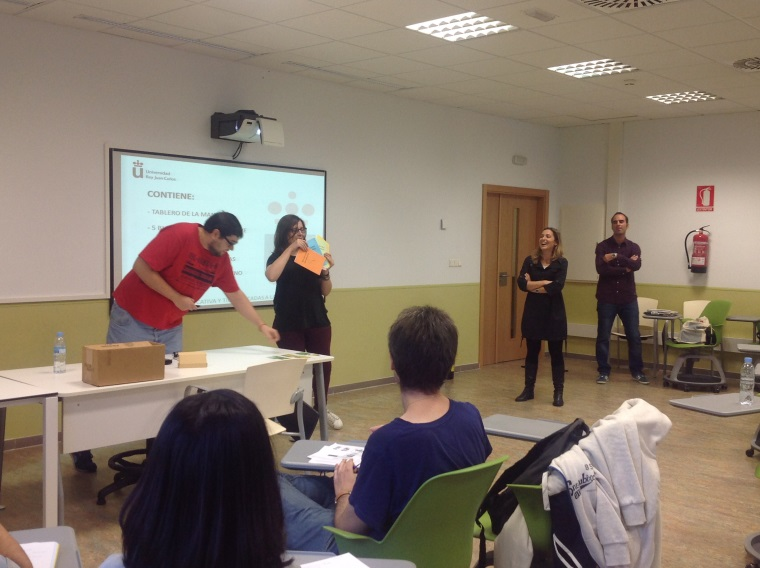
\includegraphics{img/cluedo1.jpg}
\end{figure}
La exposición estaba contextualizada en una clase para alumnos de 1º de la ESO de un IES el último día de clase antes de las vacaciones de Navidad. Durante la clase se tratará la unidad didáctica de la divisibilidad de los números primos y compuestos según aparece en el BOCM. Esta unidad didáctica suele generar mucha confusión entre los alumnos de la ESO y el grupo expositor considera que puede ser de gran interés para el alumnado.

Durante la clase se realizará un juego en el que se formarán varios equipos. Se trata de responder a una serie de preguntas en las que se premiará la rapidez en las respuestas siempre y cuando sean correctas. Por un lado el juego permitirá captar la atención de los alumnos. Por otro, el trabajo en equipo fomenta los valores de colaboración con los compañeros y el hecho de que sean preguntas cronometradas permitirá a las alumnas adaptarse a condiciones de trabajo de ciertas “presión”.

El juego se titula “Cluedo matemático”. El enunciado del juego dice así:

¡Esta noche el Señor Cero ha sido hallado asesinado en su mansión! Los detectives privados Simple y Compuesto han encontrado 99 sospechosos, pero no han podido resolver el caso. ¡Así que ahora la resolución del crimen depende de vosotros! Para ganar el juego debéis averiguar una sola cosa sobre el crimen”

Para la preparación del juego se:
\begin{itemize}
\item[1.] Coloca el tablero, hay un Hall donde empieza la acción y donde se coloca el peón, y 5 habitaciones dónde buscar pistas.

\item[2.] Prepara las tarjetas de preguntas, un tema para cada habitación.

 \item[3.] Prepara las tarjetas de pistas para descubrir al asesino, un pack de pistas por cada equipo.

\item[4.] Organiza a los alumnos en grupo, nombrando un portavoz
\end{itemize}

 \begin{figure}[h]
 \centering
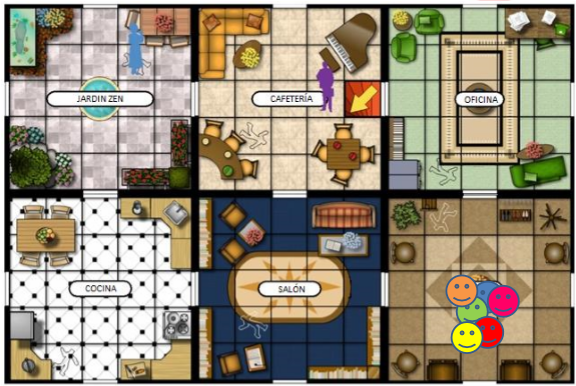
\includegraphics[scale=0.6]{img/cluedo2.jpg}
\end{figure}

Las reglas del juego son:
\begin{itemize}
\item[1.] CÓMO GANAR: ¡Resuelve el crimen!  

\item[2.] CÓMO JUGAR: En cada turno se mueve el peón a una habitación contigua, se le hace a todos los grupos la misma pregunta, se dejan 120'' para calcular la respuesta y si contestan correctamente se les da una pista sobre el asesino.

\begin{figure}[h]
\centering
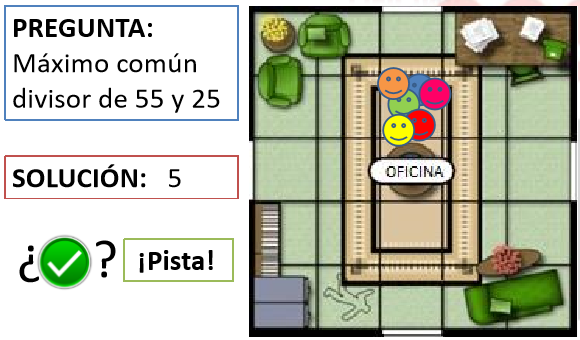
\includegraphics[scale=0.6]{img/cluedo3.jpg}
\end{figure}

\end{itemize}

 
La función principal del juego consistía en hacer preguntas por grupos y había que averiguar el número comprendido entre el 1 y el 99 a partir de una serie de pistas que se iban consiguiendo.

La exposición del grupo estuvo muy bien estructurada y demostraron que hicieron un gran trabajo de equipo.

Durante la misma explicaron que desestimaron la opción de tirar un dado, pero nosotros sí lo habríamos incluido incluyendo la posibilidad de que hubiese un rebote al tener un cronometro. Pero la opción del rebote también la descartaron.

La dificultad de las preguntas era variable por lo que es un juego muy versátil y de alto valor añadido para el aprendizaje.

Nos sorprendieron con algo novedoso al proponer analizar y evaluar el juego al final de la clase, lo que les permitirá que hubiese una mejora continua con los años. Para esta evaluación pidieron a los alumnos que contestaran a una serie de preguntas sobre lo que les ha parecido. Aunque sabemos que es difícil discernir cuando la exposición la realizas en el contexto de alumnos de secundario o en el contexto nuestro de alumnos de master, bajo nuestro punto de vista quizá sea demasiado pronto pedir la opinión a un niño de 1º de la ESO su opinión.

La exposición se ha ajustado perfectamente a los tiempos programados.


\section{Grupo 2 - Construyendo las matemáticas (21/11/2016)}


El segundo grupo está formado por:
\begin{itemize}
\item Helena Matesanz Marín 

\item Cristina Martínez Gonzalez 

\item Eliseo Virseda Alvaro 

\item Noemi Castillo Cumplido 

\item David Soria Castro 
\end{itemize}

\begin{figure}[hbtp]
\centering
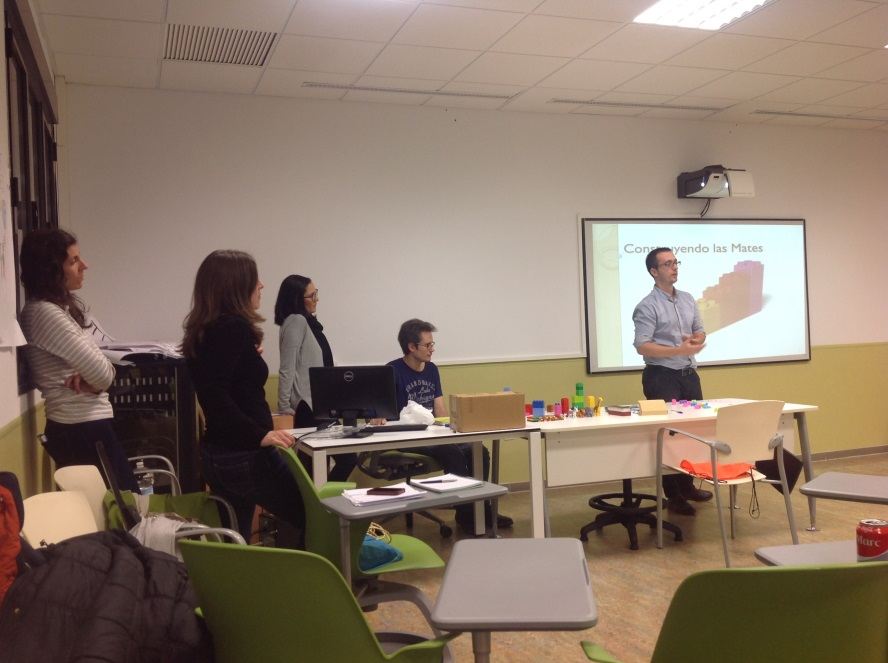
\includegraphics[scale=1]{img/lego1.jpg}
\caption{Integrantes del grupo 2.}
\end{figure}

 
La exposición consistió en explicar con un material manipulativo conocido por los alumnos, que son las piezas de LEGO, los siguientes conceptos matemáticos que en el papel pueden parecer abstractos. Los conceptos matemáticos mostrados fueron:
\begin{itemize}
\item Fracciones 

\item Estadística 

\item Máximo común divisor y mínimo común múltiplo 

\item Ecuaciones lineales simples. Despejar la x. 

\item Teorema de Pitágoras 
\end{itemize}

\begin{figure}[hbtp]
\centering
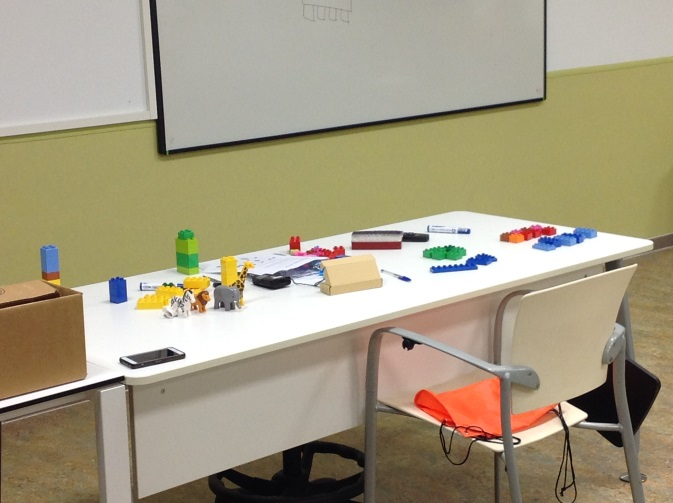
\includegraphics[scale=1]{img/lego2.jpg}
\caption{Materiales manipulativos.}
\end{figure}
 
En nuestra opinión el uso de LEGO para varios conceptos matemáticos hizo que algunos de estos temas estuvieran un poco forzados. Es decir, para el concepto de fracciones las piezas de LEGO fueron de gran utilidad al permitir de una manera visual entender el concepto de lo que es una fracción como una parte de un todo. Sin embargo consideramos que explicar el concepto de M.c.d y m.c.m con piezas de LEGO quedó un poco forzado.

Por hacer una crítica constructiva, entendemos que era un grupo de 5 alumnos, es decir, de más alumnos que el resto de grupos de clase, pero quizá hubiésemos enfocado el trabajo en uno o dos conceptos matemáticos y habríamos trabajado un par de alumnos por cada concepto para evitar explicaciones de conceptos forzadas.

La exposición estuvo muy bien estructurada con una demostración conceptual por cada alumno pero se fueron de tiempo. Es cierto que se han explicado muchos conceptos pero los alumnos no hemos colaborado con lo que se puede perder eficacia al no hacer partícipes a los alumnos. Pero también entendemos que todos tenían que hablar y que eran temas muy interesantes.

Por último, la exposición también nos sirvió para aprender que a día de hoy hay un software en una web de internet (\url{http://www.publishyourdesign.com/}) que te permite realizar diseños de LEGO en 3D con el ordenador para luego poder incluso imprimirlos con impresoras 3D.